\documentclass[a4paper,12pt]{report}

\usepackage{alltt, fancyvrb, url}
\usepackage{graphicx}
\usepackage[utf8]{inputenc}
\usepackage{float}
\usepackage{hyperref}

\hypersetup{
    colorlinks=true,
    linkcolor=black,
    filecolor=magenta,      
    urlcolor=blue,
    pdfpagemode=FullScreen,
    }

\title{Assignment 02 - \\``Smart Waste Disposal System''\\
    \large ``Embedded Systems e Internet of Things'' final report}

\author{Lorenzo Cinelli}
\date{\today}

\begin{document}

\maketitle

\tableofcontents

\chapter{Analysis}

    \section{Description}

        The system required is a smart waste disposal system for - potentially dangerous - liquids. It has to be composed by a container having some sensors to check the temperature of the waste and the filling level. It has also two leds and a screen to signal if the user can pour the waste or not in case of some problems. To pour the waste there is a door controlled by two buttons - one to open it and one to close it. 
        There is also an operator dashboard where operators can handle problems - like emptying the container - or consult information about the container. If no user is pouring waste the system waits a timeout and then goes in \textit{sleep mode}. 

        \begin{figure}[H]
        	\centering{}
        	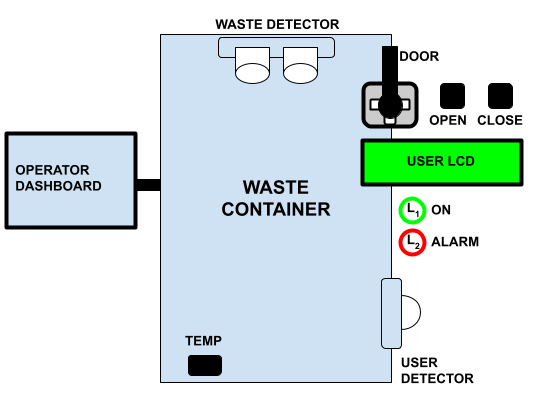
\includegraphics[width=240pt]{img/Assignment-02_SWDS-Domain.png}
        	\caption{Smart Waste Disposal System}
        	\label{img:system}
        \end{figure}
        \centerline{\href{https://docs.google.com/document/d/1iFXGmo7RVZMpJ5bxUN5ms_qFqg2B-wecRc0sfas9rQ4/edit?tab=t.0}{Here} is the complete description for the assignment.}
            
    \section{Domain Model}
    
        The waste container will manage an user detector. When an user is detected if the system was asleep it would be awaken. If for some time no one is detected the system will turn in \textit{sleep mode} in order to consume less energy.
        %
        Moreover it will manage the door, which can be opened by the user by pressing the ``Open'' button and can be closed by the user by pressing the ``Close'' button, otherwise it will close after a timeout. The door will automatically close if sensors detect that the container is full or the temperature of the liquid is too high. 
        The door can be open and close also when the operator interact with the empty or restore button in his dashboard.
        %
        Furthermore it will manage the information devices: two leds and a display.
        The green one denote that there are no problems in the container and a user can pour his waste, while the red one indicates either the container is full or the liquid inside is too hot. 
        %
        The display will show a message to the user depending on the state of the container.\\\\
        %
        The operator dashboard lets the operator see the current data of the container's sensors, which are the filling percentage and the temperature of the liquid inside. It offers also a button to empty the container, and a button to manage temperature problem inside the container. Data are stored in an history graph.\\\\
        %
        The waste container and the operator dashboard have to communicate. More specifically the dashboard will read from the waste container sensors data and will send a signal to empty or restore the container. 
            
    \section{Requirements}

        \subsection{Mandatory:}

            \begin{itemize}
                \item The system has to turn in \textit{sleep mode} if no user is detected for $T_{sleep}$ seconds. 
                \item The system has to wake up whenever an user is detected
                \item When the user presses the ``Open" button the container's door opens to let him pour waste.
                \item When the user presses the ``Close" button or $T_1$ seconds are elapsed from the opening of the container, the door will close. 
                \item The filling sensor is constantly checking for the filling level of the container, sending it to the operator dashboard. 
                \item Whenever the filling sensor detects that the container is full, it doesn't accept anymore waste until an operator empties it. If the door is open when the temperature exceeds its threshold it will immediately close. 
                \item The temperature sensor constantly checks the waste temperature sending it to the operator dashboard. 
                \item Whenever the temperature sensor detects a too high temperature in the liquid, the container doesn't accept anymore waste until the intervention of an operator. If the door is open when the temperature exceeds his threshold it will immediately close. 
                \item The display has to show different messages depending on the container's state. 
                \item When entering the pour is available it will be on the green led, while when is not available - in case of full container or waste with too high temperature - it will be on the red led.  
                \item The operator dashboard displays the current state of the container, in particular the filling percentage and the waste temperature. 
                \item An operator can empty the container through his dashboard pressing the button ``Empty the container". When the container has to empty the door will open for $T_3$ seconds. After emptying the container will be available for users. 
                \item In case of high temperature in the waste the operator can restore the container by pressing the ``Restore" button in the operator dashboard, making the container available for users.
            \end{itemize}

        \subsection{Optional:}
            
            \begin{itemize}
                \item The operator dashboard can store data to make an history graph.
            \end{itemize}

\chapter{Design}

    \section{Architecture}

        The system is composed by two modules: the container module and the operator module.
        The two modules can exchange information between each other by a serial line.\\\\
        %
        The container module is a task-based architecture. Tasks are concurrent and can interact with one another by setting and reading shared flags. Tasks are executed by a cooperative scheduler.
        More specifically there are four tasks to manage the following behaviors: container management, filling monitoring, temperature monitoring and communication with the operator dashboard.\\
        %
        Having multiple tasks offer a greater modularity, reusability and the possibility to have concurrent tasks.\\\\
        %
        The operator module is an active GUI showing the container's information and saving them to produce an history graph.
        It offers two buttons to manage issues of the container, namely the container full or the high temperature of the waste.
    
    \section{Detailed Design}

        The container module is composed by four different and concurrent tasks which are managed by a cooperative scheduler. 

        \subsection{Container management task:}

            The container management task provides to user-related actions.
            This task is described by a \texttt{synchronous finite state machine}. 

            \begin{figure}[H]
        	\centering{}
                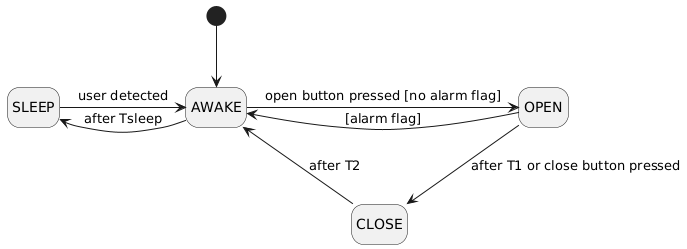
\includegraphics[width=\textwidth]{img/container_task.png}
        	\caption{Container management task}
        	\label{img:container_task}
            \end{figure}

            
            \begin{itemize}
                \item SLEEP: in this state the container is turned into \texttt{sleep mode} in order to reduce power consumption. It can be awaken by detecting an user.
                \item AWAKE: it's the initial state. In case of no actions performed by the user for $T_{sleep}$ seconds it will go in \textit{sleep} state. \\
                If there is no alarm set the container the green led is on, the red led is off and the display is showing ``press open to enter the waste''. In this case the container can go in \textit{open} state after an user pressing the open button.
                \item OPEN: in this state the container's door is open, the display showing ``press close when done'' and the user can pour his waste inside the container. If $T_1$ seconds are elapsed or the user has pressed the close button, the state will turn in \texttt{close}, closing the door.
                In case an alarm is detected by another task, and an alarm flag is set, the container will immediately turn back in \texttt{awake} state closing the door, turning on the red led and off the green one, and showing on the display an error message depending on the alarm.
                \item CLOSE: in this state the door is closed and ``waste received'' is shown on the display for $T_2$ seconds, then the container will go in \texttt{awake} state. 
            \end{itemize}

        \subsection{Filling monitoring task:}

            The filling monitoring task provides to periodically check the filling level of the container.
            This task is described by a \texttt{synchronous finite state machine}. 

            \begin{figure}[H]
        	\centering{}
                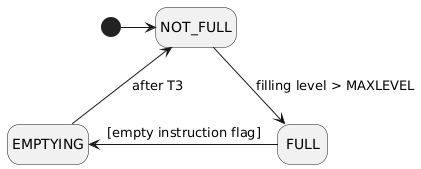
\includegraphics[width=\textwidth]{img/filling_task.png}
        	\caption{Filling monitoring task}
        	\label{img:filling_task}
            \end{figure}

            \begin{itemize}
                \item AVAILABLE: it's the initial state. It monitors the filling of the container and if it surpasses the maximum capacity of the container it turns in \texttt{full} state setting a \texttt{full alarm flag}, turning on the red led, off the green one and displaying on the scree ``container full''.
                \item FULL: in this state is checked if the \texttt{empty instruction flag} is set. In this case the state is set to \texttt{emptying}, the door is opened and the instruction flag is removed.
                \item EMPTYING: this state remains for $T_3$ seconds in order to let the container empty and then the state is set to \texttt{available} and the full alarm flag removed. If there is no other alarm flag set it will also turn on the green led, off the red one and set the default ``press open to enter the waste'' message on the display.
            \end{itemize}
        
        \subsection{Temperature monitoring task:}

            The temperature monitoring task provides to periodically check the temperature of the waste.
            This task is described by a \texttt{synchronous finite state machine}. 

            \begin{figure}[H]
        	\centering{}
                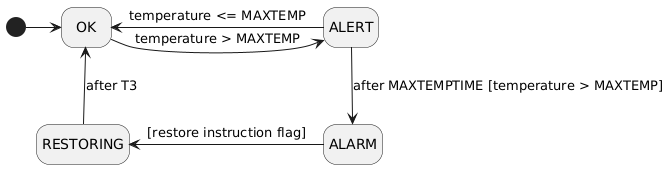
\includegraphics[width=\textwidth]{img/temperature_task.png}
        	\caption{Temperature monitoring task}
        	\label{img:temperature_task}
            \end{figure}

            \begin{itemize}
                \item OK: it's the initial state. It monitors the waste temperature and if it surpasses $MAXTEMP$ is set \texttt{alert} state. 
                \item ALERT: in this state the task checks if the temperature keeps being higher than $MAXTEMP$ for $MAXTEMPTIME$. In affirmative case the \texttt{temperature alarm flag} is set, is set the \texttt{alarm} state, the red led is turned on, the green led turned off and the message on the display is ``problem detected''. In negative case the \texttt{ok} status is put back.
                \item ALARM: in this state the task checks if the \texttt{restore instruction flag} is set and if so it puts the \texttt{restoring} state by removing the restore flag and opening the door.
                \item RESTORING: in this state the door stays open for $T_3$ seconds to let the container be emptied - in this way the temperature will no longer be a problem - and then the task's state is set to \texttt{ok}, removing the temperature alarm flag. If there is another alarm flag the display's message is changed depending on the alarm - in this case only the full alarm can be present - otherwise the green led is turned on, the red one turned off and set the default message on the display.
            \end{itemize}

        \subsection{Operator communication task:}

            This task is simpler compared to previous ones because is not described by a finite state machine.\\
            It waits on the serial line waiting for a request. The request can be:
            \begin{itemize}
                \item GET DATA: in this case it sends back on the serial line the current filling level of the container and the current temperature of the waste.
                \item EMPTY: in this case it sets the \texttt{empty instruction flag}.
                \item RESTORE: in this case it sets the \texttt{restore instruction flag}.
            \end{itemize}

\chapter{Develop}

    The system is developed in two different languages:\\\\
    %
    The container module is developed in \texttt{c++} by using \texttt{PlatformIO} IDE with \texttt{arduino} framework. It uses two external libraries: ``\href{https://github.com/johnrickman/LiquidCrystal_I2C}{LiquidCrystal\_I2C.h}'' to manage the display and ``\href{https://docs.arduino.cc/libraries/servo/}{Servo}'' to manage the servo motor.\\\\
    % 
    The operator module is developed in \texttt{python} with two threads: one for the gui and the serial communication, the other one to repaint periodically the new history graph. It uses:
    \begin{itemize}
        \item ``\href{https://pyserial.readthedocs.io/en/latest/pyserial.html}{serial}'' library to communicate through the serial line with the other module.
        \item ``\href{https://docs.python.org/3/library/threading.html}{threading}'' library to run multi thread.
        \item ``\href{https://docs.python.org/3/library/tkinter.html}{tkinter}'' library to manage the graphical part.
        \item ``\href{https://docs.python.org/3/library/time.html}{time}'' library to be able to manage time.
        \item ``\href{https://matplotlib.org/3.5.3/api/_as_gen/matplotlib.pyplot.html}{matplotlib.pyplot}'' to draw graphs.
        \item ``\href{https://pillow.readthedocs.io/en/stable/}{PIL}'' library to open images and sending to the gui.
    \end{itemize}

    \begin{figure}[H]
        \centering{}
            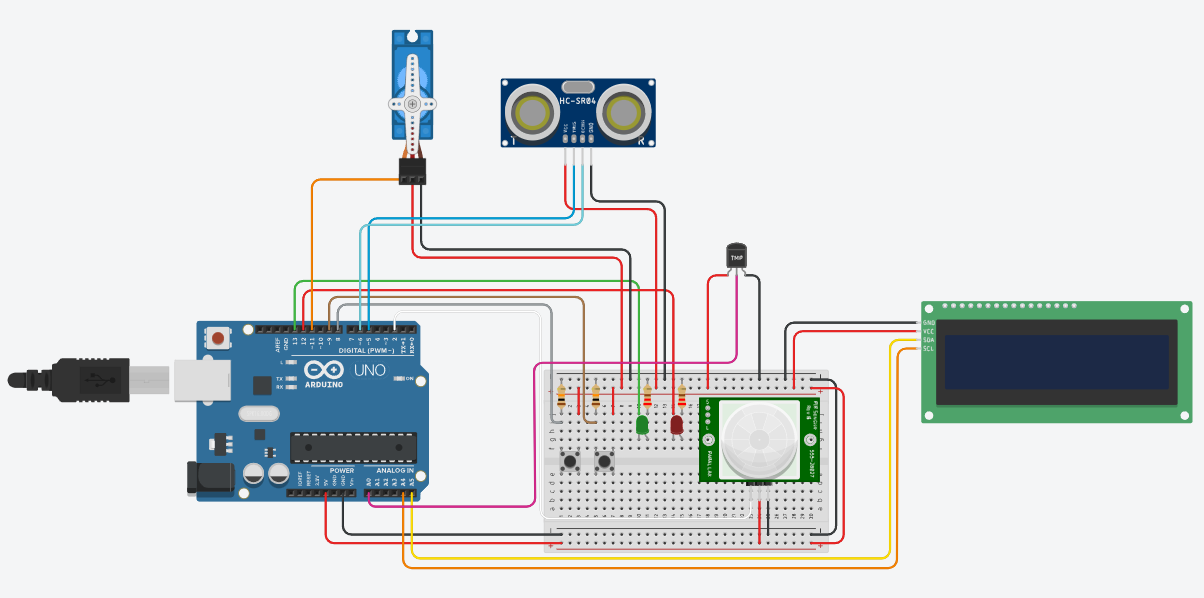
\includegraphics[width=\textwidth]{img/Assignment-02_SWDS-Schema.png}
        \caption{Circuit schema}
        \label{img:schema}
    \end{figure}
    
    \centerline{\href{https://github.com/Sansalina/IoT-assignment-02}{Here} the link to the project's GitHub repo.}
    \centerline{\href{https://drive.google.com/file/d/1d6b1z2RUoSSoMtx6eu3L8nykpJ6HNov7/view?usp=drive_link}{Here} is the link to the demonstration video.}

\end{document}